\documentclass[unicode,11pt,a4paper,oneside,numbers=endperiod,openany]{scrartcl}

\usepackage{assignment}
\usepackage{textcomp}
\usepackage{amsmath}
\usepackage{theorem}
\usepackage{algorithm,algorithmic}
\hyphenation{PageRank}
\hyphenation{PageRanks}

\newtheorem{theorem}{Theorem}
\renewcommand\thesubsection{\arabic{subsection}}
\DeclareOldFontCommand{\bf}{\normalfont\bfseries}{\mathbf}
\DeclareOldFontCommand{\it}{\normalfont\bfseries}{\mathit}


\allowdisplaybreaks

\begin{document}

\setassignment
\setduedate{Wednesday, May 26, 2021, 11.59pm}
\serieheader{Stochastic Methods}{Academic Year 2020/2021}{Prof. Dr. Illia Horenko (illia.horenko@usi.ch)}{Edoardo Vecchi (edoardo.vecchi@usi.ch)}{Assignment 5 - Solution}{[Ashutosh Singh]}

%-----------------------------------------------------------------------------------------------

\section*{Exercise 1: Irreducible and Aperiodic Markov Chains}

\begin{itemize}
	\item [(a)]
	\[
	P^{(2)} = \begin{bmatrix}
                0.75 & 0.25\\
                0.5 & 0.5
              \end{bmatrix}
    \]
              
    {Since ${p^{(2)}_{ii} > 0}$ for all i. This chain is irreducible}
    
    \begin{equation}
    {k = gcd\{t > 0: P(X_t = s_i|X_0 = s_i) > 0\}}
    \end{equation}
    
    \[
    {k = gcd\{2, 3, 4, 5,\}}
    \]
    \[
    \Rightarrow { k = 1}
    \]    
    
    {This chain is aperiodic}
    
    
    
	\item [(b)]
              
    {Even after a lot of steps  ${p^{(n)}_{21} = 0}$. This chain is not irreducible}
    
    
    \[
    {k = gcd\{1, 2, 3, 4, 5,\}}
    \]
    \[
    \Rightarrow { k = 1}
    \]    
    
    {This chain is aperiodic}
    
	
	\item [(c)]
	\[
		P^{(30)} = \begin{bmatrix}
                0.222 & 0.3333 & 0.4444\\
                0.222 & 0.3333 & 0.4444\\
                0.222 & 0.3333 & 0.4444\\
              \end{bmatrix}
    \]
              
    {Since ${p^{(2)}_{ii} > 0}$ for all i. This chain is irreducible}
\end{itemize}

%------------------------------------------------------------------------------------

\section*{Exercise 2: Tossing a Fair Coin}

\begin{flushleft}
    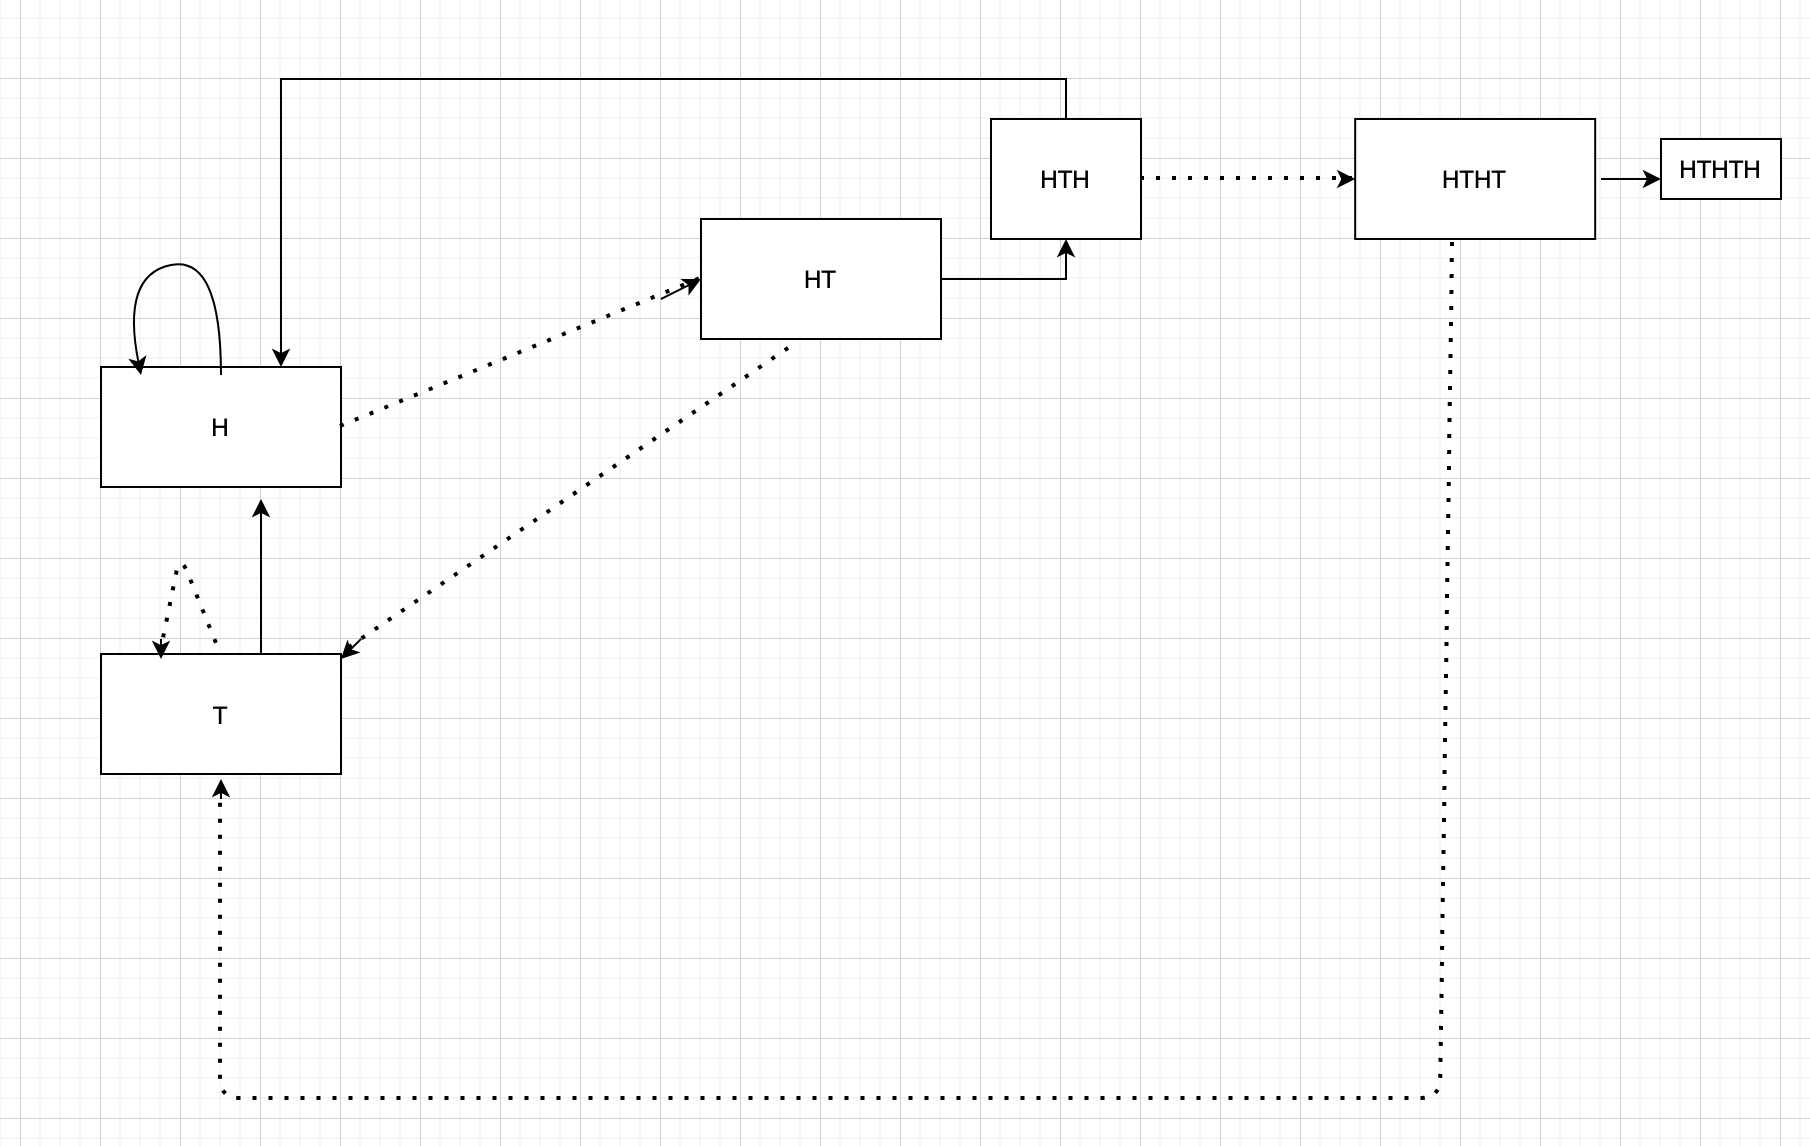
\includegraphics[width=0.80\textwidth]{markov2.png}
\end{flushleft}

{We want HTHTH. We can model this chain with 6 states}\\
\begin{itemize}
    \item Bold arrow suggest movement of chain on heads
    \item Dashed arrow suggest movement on tails
    \item Each arrow has weight $\dfrac{1}{2}$
    \item Starting from S we can move to H or T
    \item Once at T only possible states are H or T again. Because we will have to restart for the sequence we want from H.
    \item From H we can move to HT(Progression) or back to H
    \item From HT we can move to HTH(Progression) or back to T
    \item So on till we reach HTHTH
\end{itemize}

{States = \{S, H, T, HT, HTH, HTHT, HTHTH\}}



\[
		P = \begin{bmatrix}
		        0 & \dfrac{1}{2} & \dfrac{1}{2} & 0 & 0 & 0 & 0\\
		        \\
                0 & \dfrac{1}{2} & 0 & \dfrac{1}{2} & 0 & 0 & 0\\
                \\
                0 & \dfrac{1}{2} & \dfrac{1}{2} & 0 & 0 & 0 & 0\\
                \\
                0 & 0 & \dfrac{1}{2} & 0 & \dfrac{1}{2} & 0 & 0\\
                \\
                0 & \dfrac{1}{2} & 0 & 0 & 0 & \dfrac{1}{2} & 0\\
                \\
                0 & 0 & \dfrac{1}{2} & 0 & 0 & 0 & \dfrac{1}{2}\\
                \\
                0 & 0 & 0 & 0 & 0 & 0 & 1\\
              \end{bmatrix}
    \]
    

        {The last state is the absorbing state} 

    
    \[ P = 
		\begin{bmatrix}
                Q & R\\
                0 & I\\
        \end{bmatrix}
   \]
   
   \[ Q = 
		\begin{bmatrix}
		        0 & \dfrac{1}{2} & \dfrac{1}{2} & 0 & 0 & 0\\
		        \\
                0 & \dfrac{1}{2} & 0 & \dfrac{1}{2} & 0 & 0\\
                \\
                0 & \dfrac{1}{2} & \dfrac{1}{2} & 0 & 0 & 0\\
                \\
                0 & 0 & \dfrac{1}{2} & 0 & \dfrac{1}{2} & 0\\
                \\
                0 & \dfrac{1}{2} & 0 & 0 & 0 & \dfrac{1}{2}\\
                \\
                0 & 0 & \dfrac{1}{2} & 0 & 0 & 0\\
        \end{bmatrix}
   \]
   
      \[ \Phi = (I - Q)^{-1}
   \]
   
   
   \[ \tau = \Phi
        \begin{bmatrix}
                1\\
                1\\
                1\\
                1\\
                1\\
                1
        \end{bmatrix}
   \]
   \[ \tau =
        \begin{bmatrix}
                42\\
                40\\
                42\\
                38\\
                32\\
                22
        \end{bmatrix}
   \]
   
   
   {Average number of steps = $mean(\tau))$}\\
   \Rightarrow ${Average number of steps = 36}$






%-----------------------------------------------------------------------------------------

\section*{Exercise 3: Markov Process and Stationary Distribution}

    \[
		P = \begin{bmatrix}
                0 & 0.5 & 0.5\\
                0.2 & 0.5 & 0.3\\
                0.1 & 0 & 0.9\\
              \end{bmatrix}
    \]
    
    \[
		\pi^* = \pi^* P
    \]
    \[
		\pi^* = \pi^* P
    \]
    \[
		\pi^*(P - \lambda I) = 0
    \]
    
    \[
		\begin{bmatrix}
                x & y & z\\
        \end{bmatrix}
        \begin{bmatrix}
        -1 & 0.5 & 0.5\\
        0.2 & -0.5 & 0.3\\
        0.1 & 0 & -0.1\\
        \end{bmatrix}
        =
        \begin{bmatrix}
        0 & 0 & 0
        \end{bmatrix}
    \]
    
    \begin{equation}
        -x + 0.2y + 0.1z = 0
    \end{equation}
    \begin{equation}
        0.5x - 0.5y = 0
    \end{equation}
    \begin{equation}
        0.5x + 0.3y - 0.1z = 0
    \end{equation}
    
    \begin{equation}
       x = y
    \end{equation}
    \begin{equation}
       8x = z
    \end{equation}
    
    \begin{equation}
       x + y + z = 1
    \end{equation}
    
    \begin{equation}
       x + x + 8x = 1
    \end{equation}
    
    \begin{equation}
       x = 0.1
    \end{equation}
    \begin{equation}
       y = 0.1
    \end{equation}
    \begin{equation}
       z = 0.8
    \end{equation}
    
    \[ \pi^* = 
		\begin{bmatrix}
                0.1 & 0.1 & 0.8\\
        \end{bmatrix}
   \]




%-----------------------------------------------------------------------------------------

\section*{Exercise 4: Time to Absorption and Absorption Probabilities}

\begin{itemize}
	\item [(a)] 
	{No the sum of last row is greater than 1}\\
	
	\[ P_{mod} = 
		\begin{bmatrix}
                1 & 0 & 0 & 0\\
                \\
                \dfrac{1}{4} & \dfrac{1}{2} & \dfrac{1}{4} & 0\\
                \\
                0 & \dfrac{1}{3} & \dfrac{1}{3} & \dfrac{1}{3}\\
                \\
                0 & 0 & 0 & 1\\
        \end{bmatrix}
   \]
	\item [(b)] 
	{Even after a lot of steps  ${p^{(n)}_{21} = 0}$. This chain is not irreducible}\\
	
	\[
	{k = gcd\{1, 2, 3, ..\}}
	\Rightarrow{ k = 1}
	\]
	{Chain is not periodic}
	
	
	
	\item [(c)] 
	{This chain is absorbing.}
	\begin{itemize}
	    \item State-1 is absorbing.
	    \item State-4 is absorbing
	    \item State-2 and State-4 are transient.
	    \item It is possible to go from all transient states to all absorbing states
	\end{itemize}
	\item [(d)] 
	\[ P = 
		\begin{bmatrix}
                Q & R\\
                0 & I\\
        \end{bmatrix}
   \]
   
   \[ R = 
		\begin{bmatrix}
                \dfrac{1}{4} & 0\\
                \\
                0 & \dfrac{1}{3}\\
        \end{bmatrix}
   \]
   
   \[ Q = 
		\begin{bmatrix}
                \dfrac{1}{2} & \dfrac{1}{4}\\
                \\
                \dfrac{1}{3} & \dfrac{1}{3}\\
        \end{bmatrix}
   \]
   
   \[ \Phi = (I - Q)^{-1}
   \]
   
   \[ \Phi = 
        \begin{bmatrix}
                \dfrac{1}{2} & -\dfrac{1}{4}\\
                \\
                -\dfrac{1}{3} & \dfrac{2}{3}\\
        \end{bmatrix}^{-1}
   \]
   
   \[ \tau = \Phi
        \begin{bmatrix}
                1\\
                1
        \end{bmatrix}
   \]
   \[ \tau =
        \begin{bmatrix}
                3.67\\
                3.33
        \end{bmatrix}
   \]
   \begin{itemize}
       \item Starting from s2 3.67 steps on average to absorption
       \item Staring from s3 3.33 steps on average to absorption
   \end{itemize}
   
	
	\item [(e)]
	{From part-d we get R and $\Phi$}\\
	\[ B = \Phi R
    \]
    
    \[ B = 
        \begin{bmatrix}
                2/3 & 1/3\\
                1/3 & 2/3
        \end{bmatrix}
    \]
    
    \begin{itemize}
        \item Given that chain starts in s2. Probability of being absorbed in s1 is 2/3 and s4 is 1/3
         \item Given that chain starts in s3. Probability of being absorbed in s1 is 1/3 and s4 is 2/3
    \end{itemize}
	
	
\end{itemize}


%-----------------------------------------------------------------------------------------

\section*{Exercise 5: The Winner Takes It All}

\begin{itemize}
	\item [(a)] 
	\begin{flushleft}
    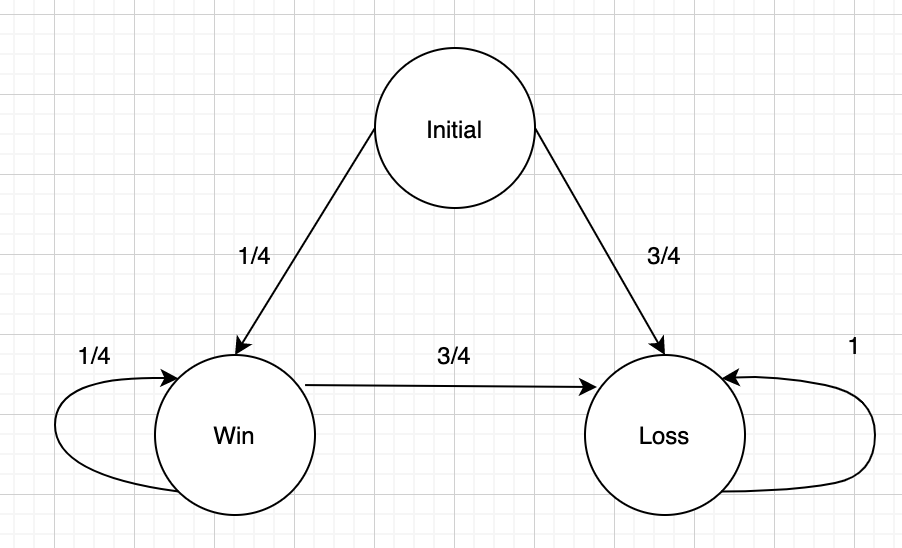
\includegraphics[width=0.60\textwidth]{markov1.png}
    \end{flushleft}
     \[ P = 
        \begin{bmatrix}
                0 & 1/4 & 3/4\\
                0 & 1/4 & 3/4\\
                0 & 0 & 1
        \end{bmatrix}
    \]
    
     \[ P^{(5)} = 
        \begin{bmatrix}
                0 & 0.000976 & 0.999\\
                0 & 0.000976 & 0.999\\
                0 & 0 & 1
        \end{bmatrix}
    \]
    
    {Since the Markov chain is Absorbing.}
    \[ \pi^* = 
		\begin{bmatrix}
                0 & 0 & 1\\
        \end{bmatrix}
   \]
    
	\item [(b)] 
	
	\[ P = 
		\begin{bmatrix}
                Q & R\\
                0 & I\\
        \end{bmatrix}
   \]
	
	\[ Q = 
        \begin{bmatrix}
                0 & 1/4\\
                0 & 1/4\\
        \end{bmatrix}
    \]
    
    \[ \Phi = (I - Q)^{-1}
   \]
   
   
   \[ \tau = \Phi
        \begin{bmatrix}
                1\\
                1
        \end{bmatrix}
   \]
   \[ \tau =
        \begin{bmatrix}
                3.67\\
                3.33
        \end{bmatrix}
   \]
    
    
	
\end{itemize}


%-----------------------------------------------------------------------------------------


\end{document}
